\documentclass[11pt]{article}
\usepackage{fullpage}
\usepackage{graphicx}
\usepackage{float}
\usepackage[hidelinks=false]{hyperref}
\usepackage{color}

\title{This is a Test}
\author{Alois}
\begin{document}

\maketitle
\clearpage
\tableofcontents
\clearpage


\section{Introduction}
\label{sec:introduction}
This is a \textbf{nice} table \ref{table:ptp_serial_results}

\begin{table}[h]
	\centering
	\begin{tabular}{|p{5cm}|p{3cm}|p{3cm}|p{3cm}|}
		\hline
		\textbf{} & \textbf{A1-A2} & \textbf{A1-A3} & \textbf{A1-A4}\\ 
		\hline
		\textbf{Number of Probes} & 36000 & 36000 & 36000\\ 
		\hline
		\textbf{Min (ns)} & -55 & -61 & -53 \\ 
		\hline
		\textbf{Max (ns)} & 47 & 49 & 54 \\ 
		\hline
		\textbf{5-Perc (ns)} & -27 & -32 & -27 \\ 
		\hline
		\textbf{25-Perc (ns)} & -7 & -14 & -9 \\ 
		\hline
		\textbf{Median (ns)} & -4& -5 & 0 \\ 
		\hline
		\textbf{75-Perc (ns)} & -1 & 4 & 11 \\ 
		\hline
		\textbf{95-Perc (ns)} & 19 & 24 & 29 \\ 
		\hline
		\textbf{99-Perc (ns)} & 30 & 34 & 39 \\ 
		\hline
		\textbf{Mean (ns)} & -4.264 & -4.714 & 0.625 \\ 
		\hline
		\textbf{StdDev (ns)} & 12.042 & 15.966 & 16.529\\ 
		\hline
		\end{tabular}
		\caption{Serial PTP Results - A1 PTP Grandmaster Clock}
		\label{table:ptp_serial_results}
		\end{table}

\textcolor{red}{Red}
\textcolor{blue}{Blue}
\color{green}text
\color{black}text

\section{Research Questions}
\label{sec:rq}
This is a \textbf{very} nice map of the internet \textsc{Scientific}. IN figure \ref{fig:glif} you can see this {\LARGE Very Good!!!}

\begin{figure}[H]
	\centering
	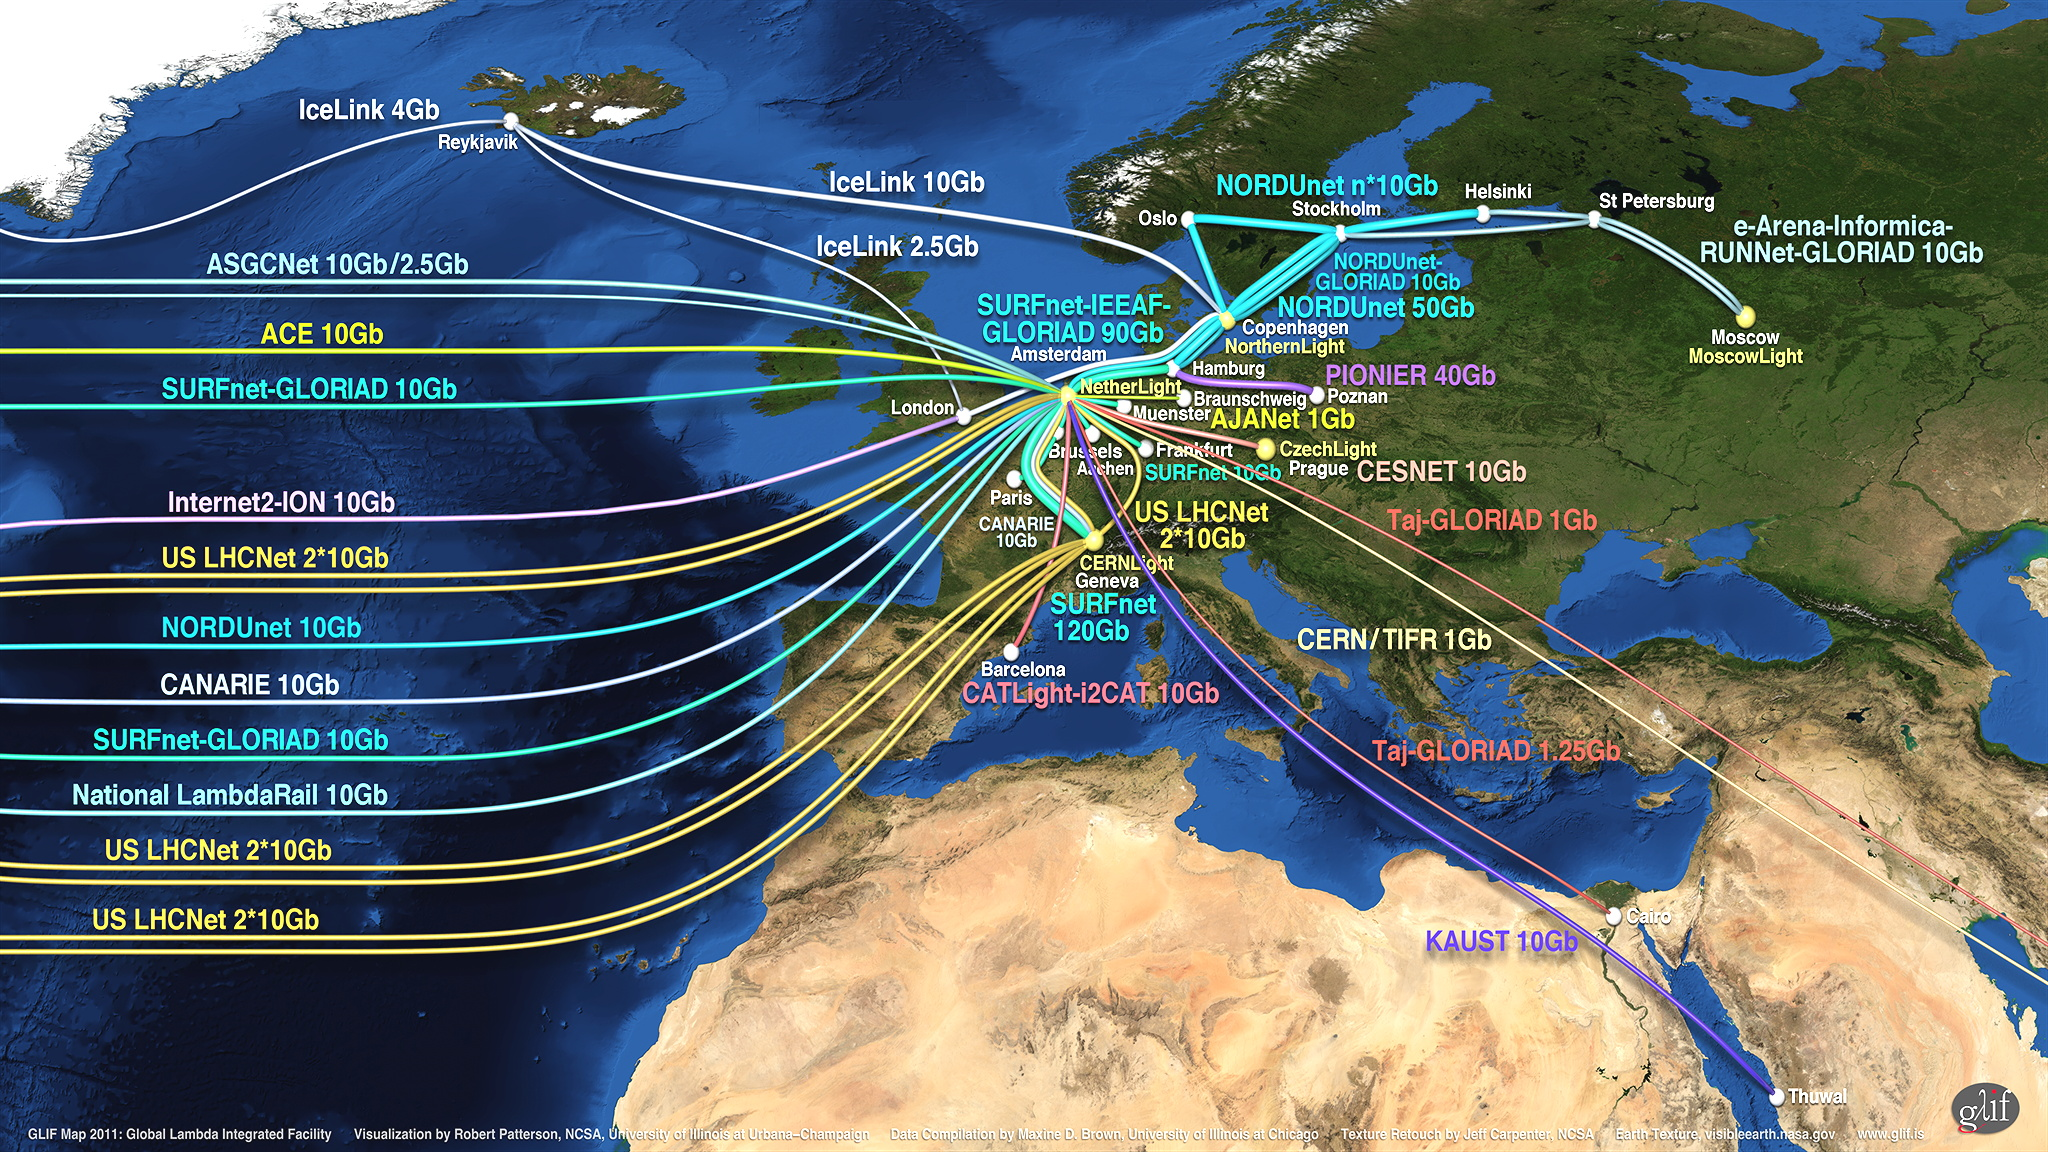
\includegraphics[width=1.0\linewidth,trim=0.0cm .0cm .0cm .0cm,clip]{pictures/GLIF_5-11_Eur_2k-enhanced.jpg}
	\caption{GLIF Map 2011}
	\label{fig:glif}
\end{figure}

And even \textit{better} {\Huge THAT!!!} this is  \LaTeX

\section{Approach}
\label{sec:approach}
\subsection*{subsection without number}
text \textbf{bold text} text. Some math: $2+2=5$
\subsection{subsection}
text \emph{emphasized text} text. \cite{WC:1953}
discovered the structure of DNA.

This is a sophisticated enumeration

\begin{enumerate}
\item{test}
\item{test3}
\end{enumerate}

\begin{itemize}
	\item testing
	\item hello world
\end{itemize}

\section{Quotes and Fonts}
\label{sec:qf}
An example of a short quote:
\begin{quote}
This is the short quote This second part is made up of two lines, if
I add enough characters I should make it. . .
\end{quote}

This is the end of the short quote

This is a math equation

\begin{equation}
k^2 \geq 1,
x = \frac{x + z/2}{y^2 +1}
\end{equation}

\begin{thebibliography}{99}
\bibitem{companion} M. Goossens, F. Mittelbach, et al. \emph{The \LaTeX\ Companion}. Addison-Wesley. 1994.
\bibitem{WC:1953} Martin Leucht.
\end{thebibliography}

\end{document}
